\documentclass[english]{article}
\newcommand{\G}{\overline{C_{2k-1}}}
\usepackage[latin9]{inputenc}
\usepackage{amsmath}
\usepackage{amssymb}
\usepackage{lmodern}
\usepackage{mathtools}
\usepackage{enumitem}
%\usepackage{natbib}
%\bibliographystyle{plainnat}
%\setcitestyle{authoryear,open={(},close={)}}
\let\avec=\vec
\renewcommand\vec{\mathbf}
\renewcommand{\d}[1]{\ensuremath{\operatorname{d}\!{#1}}}
\newcommand{\pydx}[2]{\frac{\partial #1}{\partial #2}}
\newcommand{\dydx}[2]{\frac{\d #1}{\d #2}}
\newcommand{\ddx}[1]{\frac{\d{}}{\d{#1}}}
\newcommand{\hk}{\hat{K}}
\newcommand{\hl}{\hat{\lambda}}
\newcommand{\ol}{\overline{\lambda}}
\newcommand{\om}{\overline{\mu}}
\newcommand{\all}{\text{all }}
\newcommand{\valph}{\vec{\alpha}}
\newcommand{\vbet}{\vec{\beta}}
\newcommand{\vT}{\vec{T}}
\newcommand{\vN}{\vec{N}}
\newcommand{\vB}{\vec{B}}
\newcommand{\vX}{\vec{X}}
\newcommand{\vx}{\vec {x}}
\newcommand{\vn}{\vec{n}}
\newcommand{\vxs}{\vec {x}^*}
\newcommand{\vV}{\vec{V}}
\newcommand{\vTa}{\vec{T}_\alpha}
\newcommand{\vNa}{\vec{N}_\alpha}
\newcommand{\vBa}{\vec{B}_\alpha}
\newcommand{\vTb}{\vec{T}_\beta}
\newcommand{\vNb}{\vec{N}_\beta}
\newcommand{\vBb}{\vec{B}_\beta}
\newcommand{\bvT}{\bar{\vT}}
\newcommand{\ka}{\kappa_\alpha}
\newcommand{\ta}{\tau_\alpha}
\newcommand{\kb}{\kappa_\beta}
\newcommand{\tb}{\tau_\beta}
\newcommand{\hth}{\hat{\theta}}
\newcommand{\evat}[3]{\left. #1\right|_{#2}^{#3}}
\newcommand{\prompt}[1]{\begin{prompt*}
		#1
\end{prompt*}}
\newcommand{\vy}{\vec{y}}
\DeclareMathOperator{\sech}{sech}
\DeclarePairedDelimiter\abs{\lvert}{\rvert}%
\DeclarePairedDelimiter\norm{\lVert}{\rVert}%
\newcommand{\dis}[1]{\begin{align*}
	#1
	\end{align*}}
\newcommand{\LL}{\mathcal{L}}
\newcommand{\RR}{\mathbb{R}}
\newcommand{\NN}{\mathbb{N}}
\newcommand{\ZZ}{\mathbb{Z}}
\newcommand{\QQ}{\mathbb{Q}}
\newcommand{\Ss}{\mathcal{S}}
\newcommand{\BB}{\mathcal{B}}
\usepackage{graphicx}
% Swap the definition of \abs* and \norm*, so that \abs
% and \norm resizes the size of the brackets, and the 
% starred version does not.
%\makeatletter
%\let\oldabs\abs
%\def\abs{\@ifstar{\oldabs}{\oldabs*}}
%
%\let\oldnorm\norm
%\def\norm{\@ifstar{\oldnorm}{\oldnorm*}}
%\makeatother
\newenvironment{subproof}[1][\proofname]{%
	\renewcommand{\qedsymbol}{$\blacksquare$}%
	\begin{proof}[#1]%
	}{%
	\end{proof}%
}

\usepackage{centernot}
\usepackage{dirtytalk}
\usepackage{calc}
\newcommand{\prob}[1]{\setcounter{section}{#1-1}\section{}}
\newcommand{\prt}[1]{\setcounter{subsection}{#1-1}\subsection{}}
\newcommand{\pprt}[1]{{\textit{{#1}.)}}\newline}
\renewcommand\thesubsection{\alph{subsection}}
\usepackage[sl,bf,compact]{titlesec}
\titlelabel{\thetitle.)\quad}
\DeclarePairedDelimiter\floor{\lfloor}{\rfloor}
\makeatletter

\newcommand*\pFqskip{8mu}
\catcode`,\active
\newcommand*\pFq{\begingroup
	\catcode`\,\active
	\def ,{\mskip\pFqskip\relax}%
	\dopFq
}
\catcode`\,12
\def\dopFq#1#2#3#4#5{%
	{}_{#1}F_{#2}\biggl(\genfrac..{0pt}{}{#3}{#4}|#5\biggr
	)%
	\endgroup
}
\def\res{\mathop{Res}\limits}
% Symbols \wedge and \vee from mathabx
% \DeclareFontFamily{U}{matha}{\hyphenchar\font45}
% \DeclareFontShape{U}{matha}{m}{n}{
%       <5> <6> <7> <8> <9> <10> gen * matha
%       <10.95> matha10 <12> <14.4> <17.28> <20.74> <24.88> matha12
%       }{}
% \DeclareSymbolFont{matha}{U}{matha}{m}{n}
% \DeclareMathSymbol{\wedge}         {2}{matha}{"5E}
% \DeclareMathSymbol{\vee}           {2}{matha}{"5F}
% \makeatother

%\titlelabel{(\thesubsection)}
%\titlelabel{(\thesubsection)\quad}
\usepackage{listings}
\lstloadlanguages{[5.2]Mathematica}
\usepackage{babel}
\newcommand{\ffac}[2]{{(#1)}^{\underline{#2}}}
\usepackage{color}
\usepackage{amsthm}
\newtheorem{theorem}{Theorem}[section]
%\newtheorem*{theorem*}{Theorem}[section]
\newtheorem{conj}[theorem]{Conjecture}
\newtheorem{corollary}[theorem]{Corollary}
\newtheorem{example}[theorem]{Example}
\newtheorem{lemma}[theorem]{Lemma}
\newtheorem*{lemma*}{Lemma}
\newtheorem{problem}[theorem]{Problem}
\newtheorem{proposition}[theorem]{Proposition}
\newtheorem*{prop*}{Proposition}
\newtheorem*{corollary*}{Corollary}
\newtheorem{fact}[theorem]{Fact}

\newtheorem*{claim*}{Claim}
\newcommand{\claim}[1]{\begin{claim*} #1\end{claim*}}
%organizing theorem environments by style--by the way, should we really have definitions (and notations I guess) in proposition style? it makes SO much of our text italicized, which is weird.
\theoremstyle{remark}
\newtheorem{remark}{Remark}[section]

\theoremstyle{definition}
\newtheorem{definition}[theorem]{Definition}
\newtheorem{notation}[theorem]{Notation}
\newtheorem*{notation*}{Notation}

%FINAL
\newcommand{\due}{1 November 2017} 
\RequirePackage{geometry}
\geometry{margin=.7in}
\usepackage{todonotes}
\title{Practice Test for Midterm I}
\author{David DeMark}
\date{\due}
\usepackage{fancyhdr}
\pagestyle{fancy}
\fancyhf{}
\lhead{Practice Worksheet for Midterm II}
\chead{\due}
\rhead{MATH 1271-012\&016}
\cfoot{\thepage}
% %%
%%
%%
%DRAFT

%\usepackage[left=1cm,right=4.5cm,top=2cm,bottom=1.5cm,marginparwidth=4cm]{geometry}
%\usepackage{todonotes}
% \title{MATH 8669 Homework 4-DRAFT}
% \usepackage{fancyhdr}
% \pagestyle{fancy}
% \fancyhf{}
% \rhead{David DeMark}
% \lhead{MATH 8669-Homework 4-DRAFT}
% \cfoot{\thepage}

%PROBLEM SPEFICIC

\newcommand{\lint}{\underline{\int}}
\newcommand{\uint}{\overline{\int}}
\newcommand{\hfi}{\hat{f}^{-1}}
\newcommand{\tfi}{\tilde{f}^{-1}}
\newcommand{\tsi}{\tilde{f}^{-1}}
\newcommand{\PP}{\mathcal{P}}
\newcommand{\nin}{\centernot\in}
\newcommand{\seq}[1]{({#1}_n)_{n\geq 1}}
\usepackage{array}
\newcolumntype{M}[1]{>{\centering\arraybackslash}m{#1}}
\newcolumntype{N}{@{}m{0pt}@{}}
\input ArtNouvc.fd
\newcommand*\initfamily{\usefont{U}{ArtNouvc}{xl}{n}}
\newcommand{\ild}[1]{\displaystyle{#1}}
\begin{document}

	\begin{center}{\Large\textbf{\emph{Prologue/Rapid-fire round: Midterm 1 Review}}}\end{center}
	\emph{Do not take much time on this section\textemdash if this stuff isn't automatic for you, go back to chapters 2 and 3!!}

	\prob{-2} \textbf{Compute the following limits or state they do not exist.}
	\prt{1}$\ild{\lim_{x\to 3}\frac{x^2-9}{x^2+x-12}}$
	\begin{proof}[Answer]
		$\frac{6}{7}$
	\end{proof}
	\vspace{1cm}
	\prt{2}$\ild{\lim_{x\to\infty}\frac{6x^{-2}+2x^{-1}-1}{8x^{-5}+2}}$
		\begin{proof}[Answer]
		$\frac{-1}{2}$
	\end{proof}
	\vspace{1cm}
	\prt{3} $\ild{\lim_{x\to -2}\frac{\abs{x^2-3x+10}}{x^2+5x+6}}$
		\begin{proof}[Answer]
	DNE
	\end{proof}
\vspace{3cm}
\prt{4} $\ild{\lim_{x\to \infty} \frac{(x\cos(\sqrt{x}))^2}{x^3+7}}$
	\begin{proof}[Answer]
	$0$
\end{proof}
\vspace{1cm}
\prob{-1} \textbf{Given $f(x)$, find $f'(x)$ and use it to compute $T(x)$, the tangent line to $y=f(x)$ and $x=x_0$.}
\prt{1} $\ild{f(x)= \frac{x^3+10x}{e^x}}$
\newline$x_0=1$
	\begin{proof}[Answer]
	$$f'(x)=\frac{-x^3+3x^2-10x+10}{e^x}$$
	
	$$T(x)=\frac{2(x-1)+11}{e}=\frac{2x+9}{e}$$
\end{proof}


\prt{2} $\ild{f(x)=\sqrt{e^x+\tan{x}}}$\newline$x_0=0$
	\begin{proof}[Answer]
	$$f'(x)=\frac{e^x+\sec ^2(x)}{2 \sqrt{e^x+\tan (x)}}$$
	
	$$T(x)=x+1$$
\end{proof}
\prt{3} $\ild{f(x)=\ln(x^3+3^x)}$\newline$x_0=2$
	\begin{proof}[Answer]
	$$f'(x)=\frac{3 x^2+3^x \ln (3)}{x^3+3^x}$$
	
	$$T(x)=\frac{3(4+\ln27)}{17}(x-2)+\ln 17$$
\end{proof}

\prob{0}\textbf{Use the definition of derivative to find $f'(x)$. Check your work using rules of differentiation. Also, state the domain of $f$}

$\ild{f(x)=\sqrt{2x^2-1}}$
\begin{proof}[Answer]
	$$f'(x)=\frac{x}{\sqrt{2x^2-1}}$$
(Hint: multiply by conjugate.)
\end{proof}
     
	\newpage
	\begin{center}{\Large\textbf{\emph{Implicit Differentiation and Applications (including rel8ed r8s)}}}\end{center}
	\prob{1} \textbf{Compute $\dydx{y}{x}$ in terms of $x$ and $y$ (Hint: try simplifying or otherwise manipulating the equation to make things less messy). Then, find the tangent line at the given point $(x_0,y_0)$}\newline
	$$\ild{\frac{2^{y}}{x}=2yx}\hspace{1cm}(x_0,y_0)=(1,1)$$
	\begin{proof}[Answer]
$$\dydx{y}{x}=\frac{2^y+2y}{x(\ln2)2^y-2x^3}$$ $$T(x)=\frac{2}{\ln2-1}(x-1)+1$$
	\end{proof}

\prob{2} \textbf{Use implicit differentiation to compute $f'(x)$ where $f(x)=\arccos{x^2}$ \emph{without looking up the derivative of $\arccos$.} (Hint: you should get an answer in terms of $x$ and $f(x)$ (or $y$ if you so choose). Substitute in $y=\arccos x$, then draw a triangle to simplify it to the well-known version).}
\begin{proof}[Solution]
	We start with the equation $y=\arccos(x^2)$ and apply cosine to both sides to yield $\cos y=x^2$. Differentiating, we have $-\dydx{y}{x}\sin y=2x$, or $$\dydx{y}{x}=\frac{-2x}{\sin y}$$
	We have that $y=\arccos (x^2)$, so we substitute that in:
	$$\dydx{y}{x}=\frac{-2x}{\sin(\arccos(x^2))}$$
	Recall that $\arccos$ takes as its input a ratio and spits out an angle. Let's draw a right triangle with one angle labeled as $\arccos(x^2)$ (Figure 1). Then, the ratio of the adjacent side to the hypotenuse is $x^2$, so why don't we let that adjacent side have length $x^2$ with the hypotenuse having length $1$. The Pythagorean theorem then tells us that the opposite side must have length $\sqrt{1-x^4}$.
	
	\begin{figure}[h!]\centering
		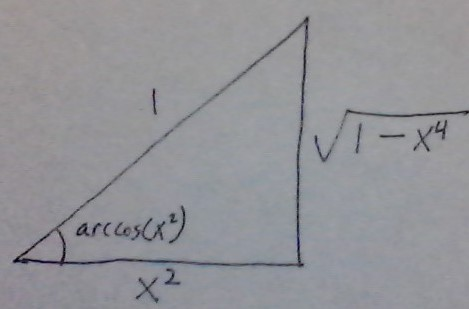
\includegraphics[scale=.5]{triangle}\caption{Our triangle, with side lenghts labeled.}
	\end{figure}
	
	 As our hypotenuse has length 1, we now have that $\sin(\arccos(x^2))=\sqrt{1-x^4}$. We can finally conclude that $$\dydx{y}{x}=\frac{-2x}{\sqrt{1-x^4}}$$
\end{proof}

%TYPE SOLUTIONS
	\prob{3}
\textbf{Compute $\dydx{y}{x}$ for $y=x^{\sin{x}}$}
\begin{proof}[Answer]
	$$\dydx{y}{x}=x^{\sin x}\left(\cos x \ln x +\frac{\sin x}{x}\right)$$
\end{proof}
\prob{4} \textbf{A weather balloon is floating at a constant altitude of 50m above level ground. It is connected by a length of rope connecting it and a spool on the ground. The balloon is floating horizontally away from its tether at a constant rate of 3 m/s. Find the rate at which the angle (in radians!) its rope makes with the ground is changing when the rope is extended to a length of 626 m. You may assume that the rope is stretched fully taut.}\begin{proof}[Answer]
$$\dydx{\theta}{t}=\frac{-150}{624^2}=\frac{-25}{64896}$$
\end{proof}
		\begin{center}{\Large\textbf{\emph{Approximations: Differentials \& Newton's Method}}}\end{center}
		\prob{5} \textbf{Use Newton's method to estimate a root to the following functions to five decimal places from the given starting point (if one is given).}
		\prt{1} $f(x)=e^x-3x$; $x_1=1.5$
		\begin{proof}[Answer]
				\begin{align*}
	x_1&=	1.5\\x_2&= 1.51236\\x_3&= 1.51213\\ x_4&=1.51213
	\end{align*}
			\end{proof}
		\prt{2} $f(x)=x^5+x^4-x^3+x^2-x+1$\begin{proof}[Answer]
			\begin{align*}
			x_1&=	-2\\x_2&= -1.96774\\x_3&= -1.96595\\ x_4&=-1.96595
			\end{align*}
		\end{proof}
	
		\prob{6} \textbf{Use Newton's method to estimate the quantity $\sqrt{3+2\sqrt[3]{4}}$}
		\begin{proof}[Answer]
			Use $f(x)=(x^2 - 3)^3 - 32=x^6-9 x^4+27 x^2-59$\begin{align*}
				x_1&=3.00000\\x_2&= 2.71605\\x_3&= 2.54997\\x_4&= 2.49156\\x_5&= 2.48499\\x_6&= 2.48491\\x_7&= 2.48491
			\end{align*}
		\end{proof}
		\prob{7} \textbf{Find $\d y$ at $x_0$ given $\d x$.}
		\prt{1} $y=x^3+1$; $x_0=2$, $\d x=.01$ (Do this without a calculator.)
		\begin{proof}[Answer]
			$\d y=.12=\frac{3}{25}$
			\end{proof}
		\prt{2} $y=\cos{(2\pi x^2)}$; $x=.4$, $\d x=.1$\begin{proof}[Answer]
			$\d y \approx -0.424406$
		\end{proof}
		\begin{center}
			{\Large\textbf{\emph{Differential Behavior: Curve Sketching \& The Mean Value Theorem}}}\end{center}
			\prob{8} \textbf{Show that $f(x)=\frac{e^x-e^{-x}}{2}$ does not have any root $x_0$ on the interval $(0,\infty)$. State which theorem you are using (if any) and justify that it may be applied.}
			\begin{proof}[Sketch]
				Proof by contradiction! Here's a step-by-step with many blanks left unfilled \begin{itemize}
				\item Show $f(0)=0$.
				\item Assume another root $x_0>0$
				\item Note $f$ is continuous \& differentiable everywhere
				\item Use Rolle's theorem/MVT to show there must be some $x_*>0$ such that $f'(x_*)=0$.
				\item Show $f'(x)$ has no roots on $(0,\infty)$.
				\item Bask in the magnificent logical power of reductio ad absurdum.
				\end{itemize}
			\end{proof}
			\prob{9}\textbf{Given $f$, sketch the curve and list any asymptotes of any type. State whether the curve has even or odd symmetry or neither. State as well the domains on which $f$ is (i) continuous (ii) increasing/decreasing (iii) concave up/down. (Hint: the functions given should factor and/or simplify surprisingly nicely.)}\prt{1}
			$\ild{f(x)=x^5-2x^3+x}$ 
			\prt{2} $\ild{f(x)=\frac{x^2+xe^{-x}+2x+e^{-x}+1}{x+1}}$\newpage
			
		
	\begin{center}{\Large\textbf{\emph{Extrema and Optimization}}}\end{center}
	\prob{10} Let $L(x)=2x+1$ and $P(x)=-15+8x-x^2$.
	\prt{1}\textbf{ Find the $x$-coordinate for the point on the graph of $y=L(x)$ which has the shortest \emph{vertical} distance to the curve $y=P(x)$. }\begin{proof}[Solution]
The \emph{vertical} distance between the two curves (i.e. the difference between the $y$-coordinates) can be given by $v(x)=\abs{L(x)-P(x)}=\abs{x^2 - 6 x + 16}$. We notice that (by the quadratic formula giving a complex result and the fact that leading coefficient is positive) that $L(x)-P(x)>0$ for all $x$, so we may safely drop the absolute value and instead minimize $v(x)=x^2-6x+16$. Taking a derivative gives $v'(x)=2x-6$, and solving that for $x$ gives $x=3$. The second derivative $v''(x)=2>0$, so this is indeed a local minimum, and as the only critical point, it must be our absolute minimum. Thus, the $x$-coordinate we're looking for is $x=3$. 		
	
	\end{proof}
	\prt{2}\textbf{ Find the $x$-coordinate for the point on the graph of $y=P(x)$ which has the shortest \emph{total} distance to the origin $(0,0)$. }\vspace{5cm}
	\begin{proof}
		The horizontal distance from $(x,P(x))$ to the origin is $x$, and the vertical distance is $P(x)$. The distance formula then gives $d(x)=\sqrt{x^2+P(x)^2}=\sqrt{x^2+(-15+8x-x^2)^2}=\sqrt{225 - 240 x + 95 x^2 - 16 x^3 + x^4}$. Then, to minimize this, we take a derivative and set it equal to zero. The chain rule gives us:$$d'(x)=\frac{2 x^3-24 x^2+95 x-120}{\sqrt{x^4-16 x^3+95 x^2-240 x+225}}$$
		
		Oh yikes, this problem is actually too hard as well--we absolutely should NOT ask you to solve a gross cubic like that at any point. My bad!!
		
		Anyway, the minimum is at $$x=-\frac{\sqrt[3]{36-\sqrt{1290}}}{6^{2/3}}-\frac{1}{\sqrt[3]{216-6 \sqrt{1290}}}+4\approx 2.60823$$
		but there is no expectation you're able to find that by hand. Sorry!
	\end{proof}
	
	\prob{11} \emph{(Go ahead and use a calculator on this one\textellipsis)}\newline\textbf{Hans is planning his workout. He plans on using a stationary bike for some time, then going for a jog. He wants to burn 600 calories over the course of his workout. He burns $50\log t_1$ calories in $t_1$ minutes on the stationary bicycle, and $75\log t_2$ calories in $t_2$ minutes jogging. What is the least amount of time he could spend working out?\footnote{physiology/exercise science/nutrition majors: yes, I know this question is physically wildly unrealistic.}}
\begin{proof}[Solution]
	We want to minimize time, with the constraint that Hans must burn 600 calories. Let $t_1$ be time biking and $t_2$ time jogging. Then, our optimization equation is $T=t_1+t_2$, and our constraint equation is $600=50\log t_1+75\log t_2$. Let's solve that for $t_2$. We have:\begin{align*}
	600-50\log t_1&=75\log t_2\\
	\implies \log t_2&=\frac{600-50\log t_1}{75}=\frac{24-2\log t_1}{3}\\
	\implies t_2&=e^{\frac{24-2\log t_1}{3}}\\&=\frac{e^8}{e^{\frac{2}{3}\log t_1}}=e^8t_1^{-\frac{2}{3}}
	\end{align*}
	Now, let's substitute that in: we get $$T(t_1)=t_1+e^8t_1^{-\frac{2}{3}}$$
	So, taking our derivative:
	$$T'(t_1)=1-\frac{2}{3}e^8t_1^{-\frac{5}{3}}$$
	All that is left to do is solve for critical points, then double-check that we do indeed have the absolute maximum (incidentally, it occurs to me now that there are no endpoints to check because I accidentally wrote this problem such that biking/jogging for very very small amounts of time burns a number of calories approaching $-\infty$\textemdash in other words, if Hans ceases biking or jogging for a minute (in fact I think he has to do both at the same time), he will suddenly take in an infinite number of calories and become a singularity, inducing a black hole. I hope Hans doesn't stop biking or jogging any time soon. Oh well, let's find some critical points)
	
	Setting $T'$ equal to $0$, we must solve \begin{align*}
		0&=1-\frac{2}{3}e^8t_1^{-\frac{5}{3}}\\
		\implies 1&=\frac{2}{3}e^8t_1^{-\frac{5}{3}}\\
		\implies \frac{3}{2e^8}&=t_1^{-\frac{5}{3}}\\
		\implies \frac{2e^8}{3}&=t_1^\frac{5}{3}\\
		\implies \left(\frac{2e^8}{3}\right)^\frac{3}{5}&=t_1\approx 95.2706
	\end{align*}
	And that is indeed our only critical point, so by our observation above, it must be our minimizing $t_1$! Indeed, $T''(t_1)=\frac{10}{9}e^8t_1^{-\frac{8}{3}}$, which is positive for any positive $t_1$, so we confirm that it is a local minimum by the second derivative test\textemdash as it is our only critical point and it is a local minimum, it must be a global minimum.
	
	Finally, let's find $t_2$ and use that to find $T$. We have from above that $t_2=e^8t_1^{-\frac{2}{3}}$. Plugging in our minimizing value of $t_1$ gives us $t_2\approx 142.906$, so Hans must slave away for $t_1+t_2\approx 238.176$ minutes. That will take forever!
\end{proof}
	\newpage

	\begin{center}{\Large\textbf{\emph{Odds \& Ends: Indeterminates and Antiderivatives}}}\end{center}
	\prob{12} \textbf{Compute the following limits.}
	\prt{1}$\ild{\lim_{x\to 1}\frac{x^6-1}{\sin(2\pi x)}}$\begin{proof}[Answer]
		$$\lim_{x\to 1}\frac{x^6-1}{\sin(2\pi x)}=\frac{3}{\pi}$$
	\end{proof}
	\prt{2}$\ild{\lim_{x\to a}\frac{\cos x \ln (x-a)}{\ln(e^x-e^a)}}$\begin{proof}[Answer]
		$$\lim_{x\to a}\frac{\cos x \ln (x-a)}{\ln (e^x-e^a)}=\cos(a)$$
	\end{proof}
	\prt{3} $\ild{\lim_{x\to \infty} \left(1+\frac{3}{x}\right)^{4x}}$
\begin{proof}[Answer] $${\lim_{x\to \infty} \left(1+\frac{3}{x}\right)^{4x}}=e^{12}$$
	\end{proof}
	\prob{13} Compute the antiderivative of $\ild{\frac{x-x^3}{\sqrt[3]{x}}}$
	
	\begin{proof}[Answer]
		We should get $\frac{3}{5}x^{5/3}-\frac{3}{11}x^{11/3}+c$
	\end{proof}
\end{document}
